% =================================================================================================
\chapter{Biološke osnove} % Main chapter title
\label{bioloskeosnove} % For referencing the chapter elsewhere, use \ref{Chapter1} 
% =================================================================================================

U ovoj sekciji biće ukratko predstavljene biološke osnove neophodne za razumevanje rada i motivacije koja stoji iza određenih njegovih elemenata.
Najpre, biće opisano šta su proteini, koje su njihove osnovne funkcije i kakva im je struktura. Potom, biće opisana svaka od struktura ponaosob, uz priložen grafički prikaz istih. Na kraju, posebno će biti opisani neuređeni proteini, njihova uloga i uzroci koji mogu dovesti do njihove pojave. 

% -------------------------------------------------------------------------------------------------
\section{Proteini}
\label{sec:proteini}
% -------------------------------------------------------------------------------------------------

Proteini (grč.~{\em protos} - $"$zauzimam prvo mesto$"$) su biološki makromolekuli neophodni za izgradnju i pravilno funkcionisanje ćelija, i igraju mnogobrojne uloge u različitim procesima koji se odvijaju unutar organizma. Predstavljaju najvažniji sastojak žive materije i utiču na brojnost i raznolikost živih bića. Specifičnost proteina je tolika da svaka biljna i životinjska vrsta ima svoje proteine, dok se, kod viših organizama, razlikovanje može uočiti i na individualnom nivou. Broj proteina u živim bićima je ogroman, na primer $E. coli$ sa $3000$ i čoveka sa $5$ miliona proteina~\cite{spasic}.\\

Proteini i peptidi su izgrađeni od $22$\footnote{Neki proteini u svom sastavu mogu da imaju $22$ različite aminokiseline. Pored $20$ standardnih aminokiselina, postoje i $2$ nestandardne i to su Selenocistein (eng.~{\em Selenocysteine}, simboli $Sec$, $U$) i Pirolizin (eng.~{\em Pyrrolysine},
simboli $Pyl$, $O$). Ove dve aminokiseline se ređe javljaju~\cite{MarijaJ}.} $L-aminokiseline$ \footnote{$L-aminokiseline$ su one sa levom prostornom konfiguracijom, analogno, postoje i $D-aminokiseline$, sa desnom} koje se javljaju u prirodi i povezani su peptidnim vezama, koje nastaju između $\alpha$-karboksilne grupe jedne aminokiseline i $\alpha$-amino grupe druge aminokiseline, pri čemu se oslobađa molekul vode~\cite{MarijaJ}. Ovim postupkom nastaje nerazgranati polipeptidni lanac izgrađen od glavnog lanca, koji se pravilno ponavlja, i međusobno različitih ogranaka. Standardna grupa aminokiselina se može podeliti na esecijalne i
neesecijalne, čiji spisak se može videti u tabeli \ref{table:1}~\cite{MarijaJ,biopathways}.\\ 
\begin{table}[h!]
\centering
	\begin{tabular}{||c c||} 
	\hline 
	Esencijalne & Neesencijalne \\ [0.5ex] 
	\hline\hline
	Arginin & Alanin \\ 
	\hline
	Histidin & Asparagin \\
	\hline
	Leucin & Asparaginska kiselina\\
	\hline
	Izoleucin & Cistein \\
	\hline
	Lizin & Glutaminska kiselina \\ [1ex] 
	\hline
	Metionin & Glutamin \\ [1ex] 
	\hline
	Fenilalanin & Glicin \\ [1ex] 
	\hline
	Treonin & Prolin \\ [1ex] 
	\hline
	Triptofan & Serin \\ [1ex] 
	\hline
	Valin & Tirozin \\ [1ex] 
	\hline
	\end{tabular}
\caption{Spisak esencijalnih i neesencijalnih aminokiselina}
\label{table:1}
\end{table}


Svaki molekul proteina nastaje u ćeliji živog organizma. Proteinski lanac se sastoji od određenog broja i vrsti aminokiselina poređanih po specifičnom redosledu. Ovaj redosled je unapred određen i zavisi od redosleda nukleotida u dezoksiribonukleinskoj kiselini (DNK), odnosno gena, koji predstavljaju trojke nukleotida. Svakoj takvoj trojci jedinstveno je pridružena po jedna aminokiselina na osnovu genetskog koda. Proces kojim se enkodirana informacija prevodi iz DNK u niz aminokiselina u proteinskom lancu, posredstvom glasničke (eng.~{\em messenger}) ribonukleinske kiseline (RNK) i transportne (eng.~{\em transfer}) RNK, naziva se genska ekspresija. Proces sinteze proteina predstavlja \textit{centralnu dogmu molekularne biologije}, čiji se prikaz može videti na slici \ref{fig:dogma}~\cite{JKd}.

\begin{figure}[h]
	\centering
    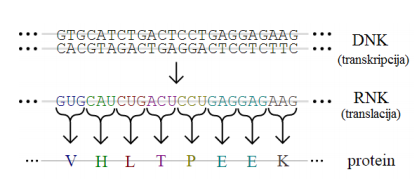
\includegraphics[width=0.5\textwidth]{Figures/BO/dogma.png}
    \caption{Prikaz centralne dogme molekularne biologije~\cite{JKd}}
    \label{fig:dogma}
\end{figure}

\subsection{Funkcije i osobine proteina}
%~\cite{JKd}
Pri istraživanju bioloških procesa neophodno je znati i dobro razumeti funkcije proteina, što se posebno može uočiti kod proučavanja oboljenja ljudi, ako se u obzir uzme činjenica da se mnoga oboljenja pojavljuju kao posledica funkcionalnih mutacija. Proteini su biološki najaktivniji molekuli sa velikim brojem esencijalnih funkcija koje se dele na:
\begin{itemize}
\item dinamičke, od kojih su najvažnije:
\begin{enumerate} 
\item transportna - prenos molekula (poput kiseonika, gvožđa, lipida) i hormona od mesta sinteze do mesta delovanja,
\item biološka - regulacija metaboličkih procesa u ćeliji, kontrola i regulacija transkripcije gena i translacija,
\item katalizatorska - biološka katalizacija \footnote{Katalizacija predstavlja proces povećavanja brzina reakcija},
\item zaštitna - keratin, koagulacija krvi,
\item održavanje zapremine tečnosti u organizmu,
\end{enumerate}
\item strukturne, od kojih su najvažnije:
\begin{enumerate}
\item obezbeđivanje čvrstine i elastičnosti organa,
\item davanje oblika organizmu,
\item izgradnja strukturnih elemenata ćelije i
\item bitna uloga u kontraktilnim i pokretnim elementima organizma.
\end{enumerate}
\end{itemize} 

Postoji nekoliko karakteristika proteina:
\begin{itemize}
\item grade kompleksna jedinjenja sa različitim supstancama po principu strukturne komplementarnosti i  
\item poseduju visoku osetljivost na različite agense koji ih denaturišu \footnote{Denaturacija proteina je proces koji izaziva promene u strukturi proteina, čime se menja i njihov fiziološki uticaj.}. Neki od najčešćih agenasa su: visoka temperatura, pritisak, mehaničko tretiranje, dejstvo kiselina, baza, organskih rastvarača, materija, itd.~\cite{spasic,JKd}.
\end{itemize}
 
\subsection{Struktura proteina}
Struktura proteina zavisi od rasporeda aminokiselina i utiče na njegovu funkciju. Trodimenzionalna struktura, koja se smatra najstabilnijom, formira se presavijanjem polipeptidnog lanca na različite načine. Unutrašnjost takve strukture ima visoku gustinu, pa polipeptidni lanac ne dopušta promene u sastavu i zahteva prisustvo aminokiselina tačno određene veličine. Uobičajena raspodela aminokiselina u proteinima je daleko od ravnomerne. Neke aminokiseline se javljaju mnogo češće od ostalih, na primer, leucin se pojavljuje devet puta više od triptofana.
%~\cite{biopathways,spasic}
Proteinsku strukturu održavaju različite vrste kovalentnih i nekovalentnih interakcija između hemijskih jedinjenja, na primer: vodonične, jonske, elektrostatičke, dipolne, itd.. Nabiranjem i uvijanjem lanaca kreiraju se različiti oblici proteina: vlaknasti, globularni ili eliptični. Ako mutacija dovede do toga da aminokiselina sa malim bočnim lancem bude zamenjena aminokiselinom sa velikim, pojaviće se problem sa formiranjem trodimenzionalne strukture. Ako bi se, pak, velika aminokiselina zamenila sa malom, pojavio bi se prazan prostor, što bi moglo dovesti do destabilizacije molekula proteina~\cite{spasic,biopathways,medbio}. \\
U molekulima proteina postoji hijerarhijska strukturalna organizacija u četiri nivoa:
\begin{enumerate}
\item primarna,
\item sekundarna,
\item tercijarna i
\item kvaternarna.
\end{enumerate}
Na slici \ref{fig:structures} se može videti opšti prikaz mogućih struktura proteina, a na drugoj \ref{fig:structures2} šematski prikaz~\cite{spasic}.
\begin{figure}[h]
	\centering
    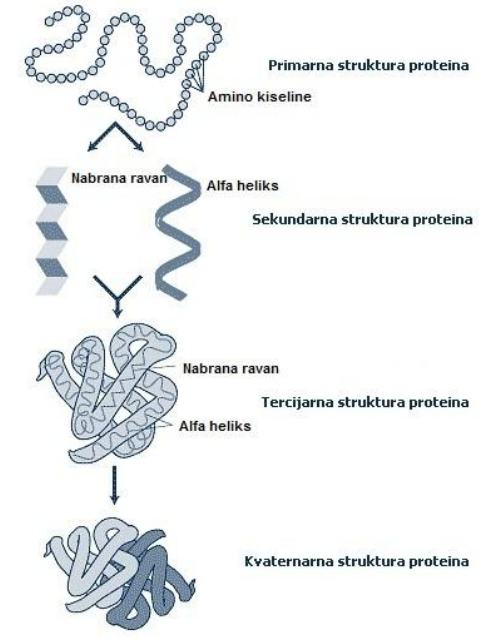
\includegraphics[width=0.5\textwidth]{Figures/BO/protein_structures.png}
    \caption{Prikaz struktura proteina}
    \label{fig:structures}
\end{figure}
\begin{figure}[h]
	\centering
    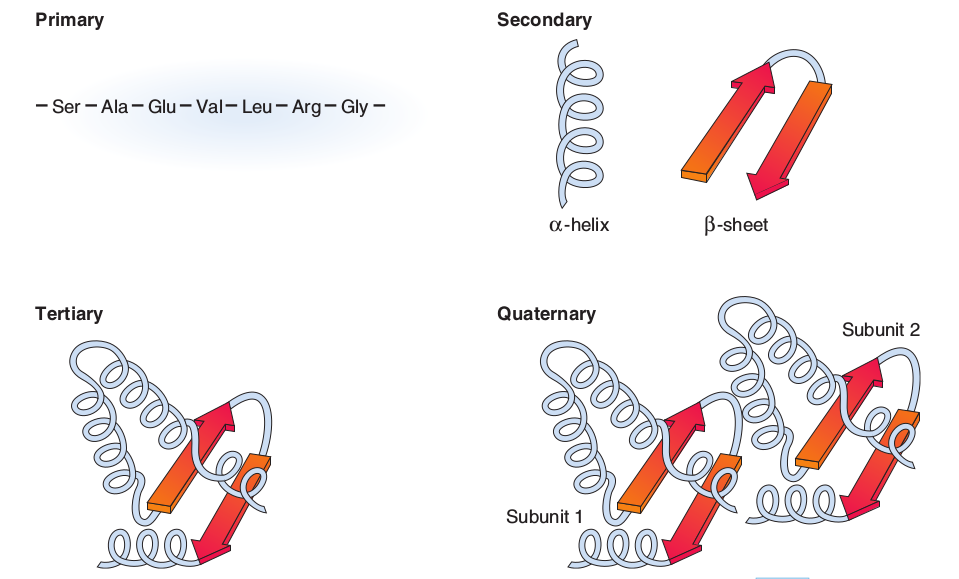
\includegraphics[width=1\textwidth]{Figures/BO/structure_schema.png}
    \caption{Šematski prikaz struktura proteina~\cite{bmbg}}
    \label{fig:structures2}
\end{figure}
\subparagraph{Primarna struktura}
Predstavlja s\^amu sekvencu aminokiselina\footnote{Redosled kojim su aminokiseline poređane u nekom polipeptidu se zove sekvenca aminokiselina~\cite{spasic}.} koje učestvuju u izgradnji proteina. Ova struktura ima ključni značaj za određivanje funkcije proteina zbog interakcija koje se javljaju između bočnih lanaca aminokiselina, a koji utiču na trodimenzionalnu strukturu. Proteini koji poseduju sličnu sekvencu aminokiselina nazivaju se $homologi$, a poređenje sekvenci među takvim proteinima može ukazati na genetsku relaciju između različitih vrsta.Prikaz izgleda primarne strukture na primeru insulina kod čoveka se vidi na slici \ref{fig:insulin}~\cite{spasic}.\\
\begin{figure}[h]
	\centering
    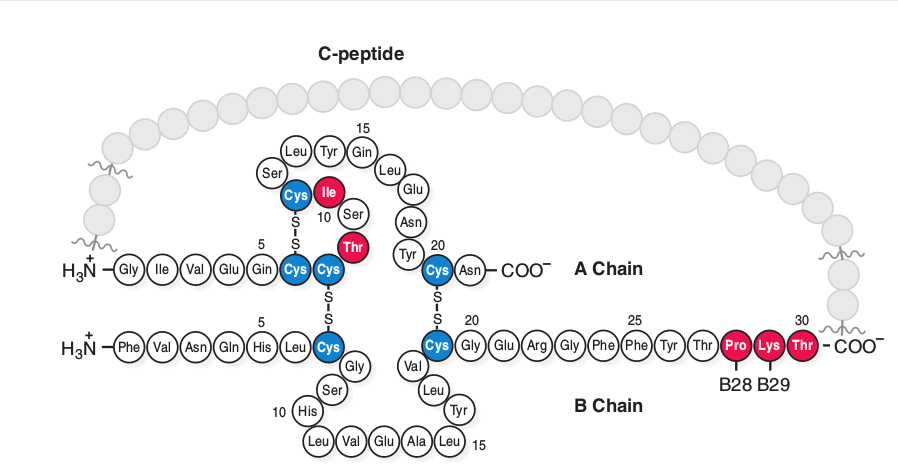
\includegraphics[width=1\textwidth]{Figures/BO/insulin.png}
    \caption{Prikaz primarne strukture~\cite{bmbg}}
    \label{fig:insulin}
\end{figure}

Mnoge genetske bolesti rezultuju u proteinima sa poremećenim redosledom aminokiselina, što uzrokuje nepravilno presavijanje i gubitak ili nemogućnost normalnog funkcionisanja. Ukoliko su nam poznate strukture normalnih i mutiranih proteina, te informacije možemo iskoristiti za dijagnostikovanje ili proučavanje bolesti. Promene u primarnoj strukturi mogu imati uticaja i na više nivoe proteinskih struktura. Takve promene često dovode do lošeg presavijanja proteina i mogu dovesti do njegovog gubitka funkcije~\cite{flash,lippincott}.

\subparagraph{Sekundarna struktura}
Odnosi se na oblik koji protein zauzima u prostoru i označava pravilno pojavljivanje ponavljanog prostornog rasporeda primarne strukture, u jednoj dimenziji. Ovu strukturu čini nekoliko različitih oblika, od kojih su najčešći $\alpha$-heliks i $\beta$-presavijena traka (ili $\beta$-struktura), a čest je i tzv. $\beta$-okret~\cite{spasic,medbio}.\\
\textbf{$\alpha$-heliks} - tip sekundarne strukture kod kog se gusto pakovani polipeptidni lanac spiralno uvrće. Karakteriše se brojem peptidnih jedinica po okretu i rastojanjem između dva okreta. Spada pod energetski najsiromašnije, a time, i najstabilnije strukture proteina. Heliks mogu obrazovati i $L-$ i $D-$ aminokiseline, pa postoje i dva tipa heliksa: levostrani i desnostrani. Prikaz izgleda $\alpha$-heliksa se vidi na slici \ref{fig:aheliks}~\cite{spasic}.
\begin{figure}[h]
	\centering
    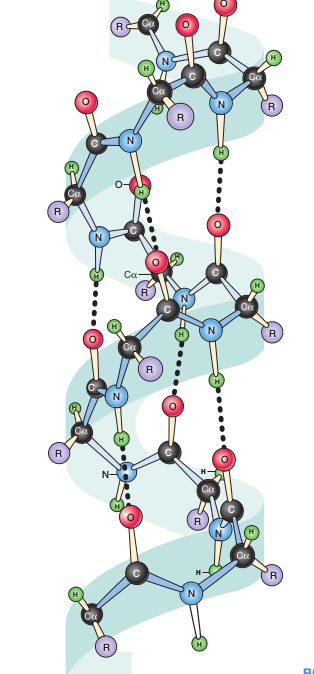
\includegraphics[width=0.25\textwidth]{Figures/BO/ahelix.png}
    \caption{Prikaz $\alpha$-heliksa~\cite{bmbg}}
    \label{fig:aheliks}
\end{figure}
 \\
\textbf{$\beta$-struktura} - Za razliku od $\alpha$-heliksa, sastoji se od dva ili više peptidnih lanaca, ili segmenata polipeptidnih lanaca, a obrazuje se kada se ovakvi tipovi lanca povežu uzdužno. Postoje dva tipa $\beta$-struktura: paralelna i antiparalelna. Prikaz izgleda $\beta$-strukture se vidi na slici \ref{fig:beta}~\cite{spasic}.\\

\begin{figure}[h]
	\centering
    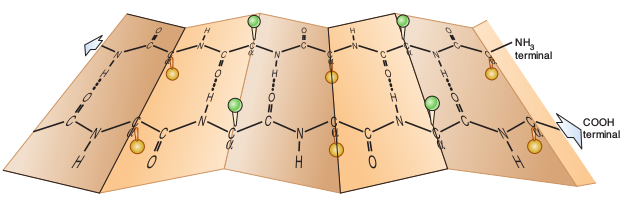
\includegraphics[width=1\textwidth]{Figures/BO/beta.png}
    \caption{Prikaz $\beta$-strukture~\cite{bmbg}}
    \label{fig:beta}
\end{figure}
\textbf{$\beta$-okreti} - obrću pravac polipeptidnog lanca praveći kompaktan globularan oblik~\cite{lippincott}. 
 
Prikaz izgleda sekundarnih struktura se nalazi na slici \ref{fig:ab}.
\begin{figure}[h]
	\centering
    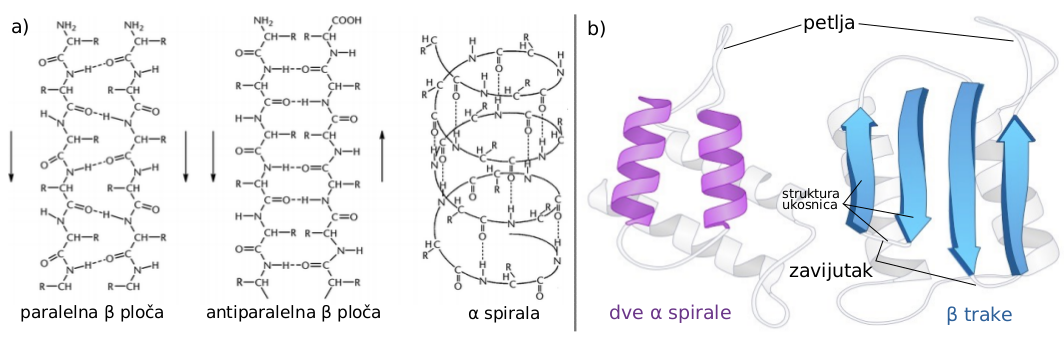
\includegraphics[width=1\textwidth]{Figures/BO/sec_structure.png}
    \caption{Prikaz sekundarnih struktura~\cite{Vinterhalter}}
    \label{fig:ab}
\end{figure}
 

\subparagraph{Tercijarna struktura}
Podrazumeva unutarmolekularno slaganje polipeptidnog lanca u kompaktnu trodimenzionalnu strukturu specifičnog oblika, koja nastaje prostornim organizovanjem polipeptidnog lanca, koji već poseduje sekundarnu strukturu. Na taj način se približavaju ostaci aminokiselina koji su udaljeni u primarnoj strukturi. Proteini koji imaju ovakvu strukturu su globularni i kompaktni sa velikom gustinom u središtu~\cite{spasic,medbio}.
\subparagraph{Kvaternarna struktura}
Predstavlja agregaciju više peptidnih lanaca u molekulu proteina. Mnogi proteini, posebno oni velike mase, izgrađeni su od nekoliko polipeptidnih lanaca. Svaka takva komponenta naziva se $podjedinica$ ili $protomer$. Oni mogu biti identični\footnote{Tada takve proteine nazivamo $oligomerima$} ili se razlikovati prema strukturi. Ovakav raspored dovodi do brzog i efikasnog transfera supstrata od jednog aktivnog centra enzima do drugog~\cite{spasic,medbio}.
 
\subsection{Savijanje proteina}
Interakcije između lanaca aminokiselina koji se nalaze sa strane, određuju kako se dugački polipeptidni lanac presavija u trodimenzionalni oblik funkcionalnog proteina. Presavijanje proteina koje se događa u ćeliji traje od nekoliko sekundi do nekoliko minuta. 
Na slici \ref{fig:folding} se može videti opšti prikaz savijanja proteina.
\begin{figure}[h]
	\centering
    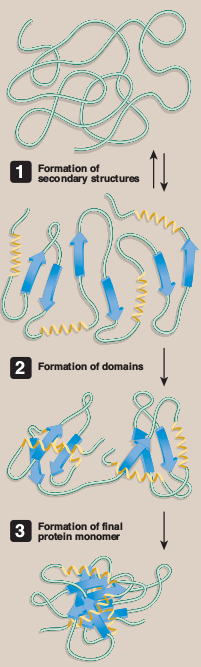
\includegraphics[width=0.25\textwidth]{Figures/BO/protein_folding.png}
    \caption{Prikaz savijanja proteina~\cite{lippincott}}
    \label{fig:folding}
\end{figure}

\subsection{Denaturacija proteina}
Denaturisanje proteina rezultuje u odvijanju i dezorganizaciji proteinske sekundarne i tercijarne strukture. Pod idealnim uslovima, denaturisanje proteina može biti $reverzibilno$. To znači da bi se protein, pri prestanku delovanja agenasa, vratio u normalno stanje. Međutim, većina proteina ostaje trajno neuređena. O neuređenosti proteina biće više reči u nastavku.\\
Jedno od objašnjenja zašto se protein ne vraća u originalno stanje se sastoji u tome da protein počinje sa savijanjem pre nego što se izvrši sinteza celog lanca. Osim toga, specijalizovana grupa pomoćnih proteina (engl. $chaperones$) je neophodna za pravilno savijanje mnogih vrsta proteina. Ovi pomoćni proteini interaguju sa polipeptidima u nekoliko faza tokom procesa savijanja, imaju ulogu u tome da održavaju protein nesavijenim dok sinteza nije gotova, ili imaju ulogu katalizatora. Loše savijanje proteina može dovesti do različitih bolesti kao što su: amiloidna bolest ili Prionova bolest~\cite{lippincott}.

% -------------------------------------------------------------------------------------------------
\section{Neuređenost proteina}
% -------------------------------------------------------------------------------------------------

Eksperimentalnim utvrđivanjem sekundarne strukture proteina (koje će biti detaljnije opisano u \ref{eksperimentalno}) uočeno je da se neretko, pod određenim fiziološkim uslovima, javljaju proteini sa trodimenzionalnom strukturom koja nije dobro definisana. Usled velikog broja termina koji se koriste za opisivanje ovakvih proteina: prirodno/suštinski neuređeni, nesavijeni, denaturisani ili reomorfni proteini (eng.~{\em intrinsically disordered/ unfolded/ unstructured}), u ovom radu, biće korišćen samo kraći termin - neuređeni proteini. \\
Neuređenost predstavlja inherentno\footnote{Inherentno = nasleđeno} svojstvo sekvence. Neuređen može biti ceo protein, a mogu biti neuređeni određeni regioni proteina različitih dužina. Kao posledica, ovakve proteine nazivamo inherentno neuređenim proteinima, skraćeno IDP\footnote{eng.~{\em Intrinsically Disordered Proteins}}, a ako su u pitanju neuređeni, ali funkcionalni, regioni, onda je skraćenica IDPr\footnote{eng.~{\em Intrinsically Disordered Protein Regions}}. Statističkom analizom došlo se do zaključka da se aminokiseline mogu klasterovati na dve grupe: 
\begin{enumerate}
\item aminokiseline koje promovišu uređenost (eng.~{\em order promoting}) i
\item aminokiseline koje promovišu neuređenost (eng.~{\em disorder promoting}).
\end{enumerate}
Neuređene proteine ili neuređene regione je teško kategorizovati, a jedan od opštih opisa strukture dat je kao kombinacija više tipova foldona\footnote{Foldon ostaje u originalnom nazivu, kao posledica manjka literature.~\cite{Vinterhalter}}:
\begin{itemize}
\item foldon (eng.~{\em foldon}) je nezavisno organizujuća jedinica(region) proteina,
\item indukativni foldon (eng.~{\em inducible foldon}) je neuređeni region proteina koji savijanje lanca postiže barem delom vezivajući se za partnera,
\item ne-foldon (eng.~{\em non-foldon}) je neuređeni region proteina koji nikada ne postiže uređenost,
\item polu-foldon (eng.~{\em semi-foldon}) je neuređeni region proteina koji ostaje polovično neuređen i nakon vezivanja za partnera, i 
\item anti-foldon (eng.~{\em unfoldon}) je region proteina koji iz uređenog prelazi u neuređeno stanje u cilju izvršavanja neke funkcije.
\end{itemize}

Postoji nekoliko mogućih stanja (oblika) u kojima se protein može naći. Ova stanja i prelazi između njih(neki proteini mogu prelaziti iz neuređenog u uređeno stanje, i obratno), prema {\em hipotezi proteinskog trojstva}, utiču na funkciju proteina. Svaki od mogućih oblika proteina može biti njegovo prirodno stanje i imati uticaja na njegovu ulogu u ćeliji. Proteini se mogu pojavljivati u raznim oblicima:
\begin{enumerate}
\item uređen protein,
\item topljiva globula (eng.~{\em molten globule}),
\item pre-topljiva globula (eng.~{\em pre-molten globule}) i 
\item nasumično klupko (eng.~{\em random coil}).
\end{enumerate}


Neuređenost proteina se utvrđuje eksperimentalno, laboratorijskim analizama, ili uz pomoć prediktora za automatsko utvrđivanje neuređenosti~\cite{JKd,IDP,IDPIDPr,DPC}. 

\subsection{Eksperimentalno ispitivanje neuređenosti proteina}
\label{eksperimentalno}
Eksperimentalno utvrđivanje neuređenosti proteina podrazumeva laboratorijsko utvrđivanje neuređenosti korišćenjem raznih biofizičkih i biohemijskih tehnika i njihovih kombinacija. Ono spada u veoma skupe i spore metode koje ne mogu da odgovore na izazove akademije i industrije. Uprkos tome, razvijen je veliki broj metoda za karakterizaciju strukture i osobina proteina. Svaka eksperimentalna metoda karakteriše se raznim prednostima manama i nivoom pouzdanosti, zbog čega je najbolje kombinovati dobijene rezultate. Naredne eksperimentalne, biofizičke i biohemijske, tehnike su najčešće u ispitivanju neuređenosti proteina~\cite{IDP,JKd}:
\begin{itemize}
\item Kristalografija X-zracima(eng.~{\em X-ray crystallography}),
\item Spektroskopija Nuklearnom Magnetnom Rezonancom (eng.~{\em NMR spectroscopy}),
\item Cirkularni dihroizam (eng.~{\em Circular dichroism (CD) spectroscopy}),
\item Osetljivost na proteolizu (eng.~{\em Sensitivity to proteolysis}),
\item Ramanova optička aktivnost, itd. 
\end{itemize}

\subsection{Računarsko ispitivanje neuređenosti proteina}

Kao posledica osobina eksperimentalnog ispitivanja neuređenosti, veliki napori su uloženi u razvoj prediktora za računarsko utvrđivanje neuređenosti proteina. Ovi prediktori uz pomoć računara, korišćenjem tehnike mašinskog učenja, vrše utvrđivanje neuređenosti proteina. Iz godine u godinu, broj ovih prediktora je sve veći, a u poslednje vreme se radi i na kreiranju metaprediktora, koji predviđanje vrše kombinovanjem više tehnika. O ovoj vrsti predikcije biće više reči u narednom poglavlju.\\
